\subsection{The Basics} 

%\DTMnewdatestyle{dateupdated}{〈definition 〉

Answers to M\Alph{subsection} problems are on page \pageref{the_basics_prob_answers}.  \textbf{\textcolor{red}{Updated \DTMnow.}}

%--------------------------------------------------------------------------------------------------------------
\begin{Exercise}[difficulty=1]
If you haven't done so already, please read the following documents on Blackboard under ``Course Information:''
\begin{itemize}[nosep]
\item The Syllabus
\item ``On Working Together Honestly''
\item About Lab Notebooks
\item Why no equation sheets
\end{itemize}
(a)~If you could change any aspect of these course policies (or anything else about the course, I guess), what would you change?  You must make at least one suggestion for a change; no fair just answering that you're fine with whatever's currently there.  (b)~How serious are you about this request?  (Are you just suggesting a change because it was required, or because you genuinely think it would improve the course?)
\end{Exercise}

%--------------------------------------------------------------------------------------------------------------
\begin{minipage}{0.7\textwidth}
\begin{Exercise}
A student wants to find the internal resistance of a standard, size-AA battery.  With no load resistor connected, the voltage across the terminals of the battery is 1.55~V.  But when the battery is connected to a load resistor of 10~$\Omega$ (as shown on the right) the voltage across the load resistor is 1.47~V.  What is the internal resistance of the battery?
\end{Exercise}
\begin{Answer}
0.544~$\Omega$ The circuit is built correctly and the output is within the range expected for the tolerances of the components. The circuit is built correctly and the output is within the range expected for the tolerances of the components. The circuit is built correctly and the output is within the range expected for the tolerances of the components.
\end{Answer}
\end{minipage}
\begin{minipage}{0.30\textwidth - 5pt}
\hfill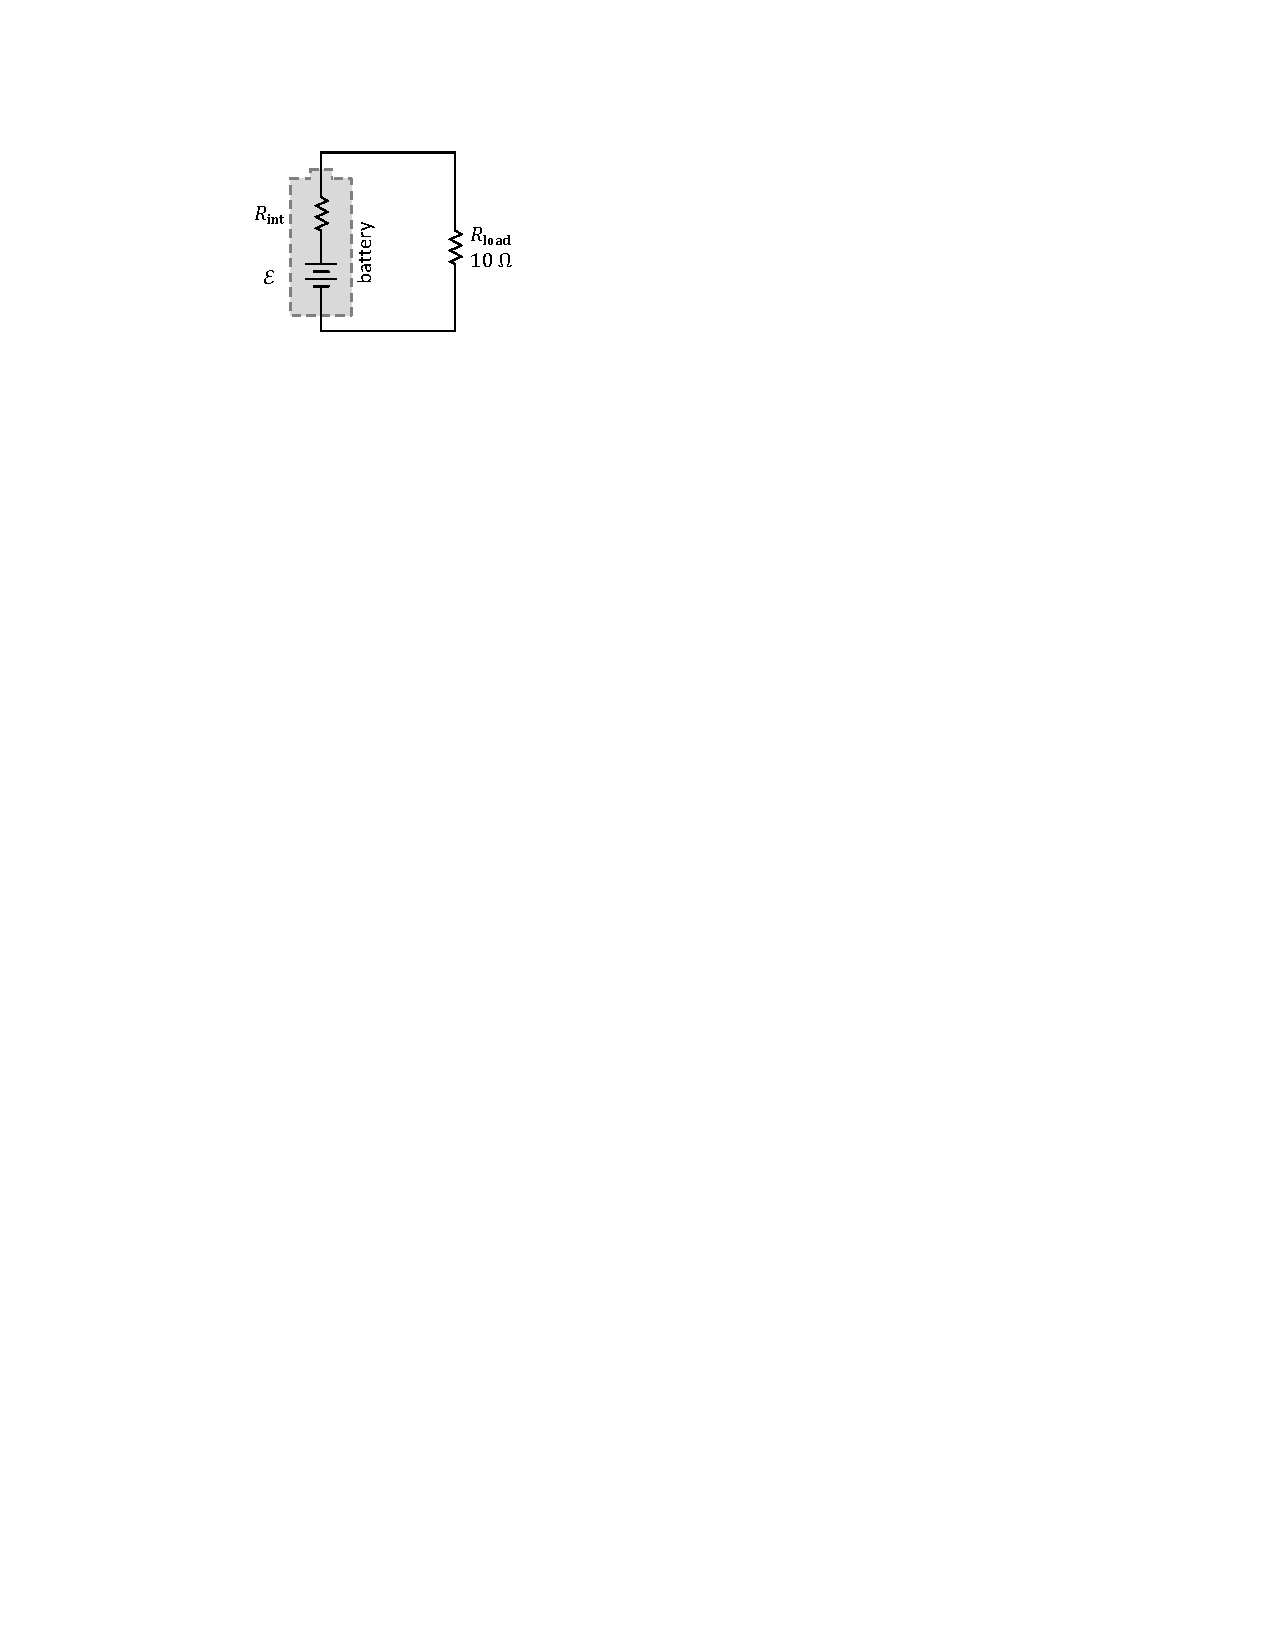
\includegraphics{M_problems/the_basics/real_battery_10ohms.pdf}
\end{minipage}

%--------------------------------------------------------------------------------------------------------------
\begin{Exercise}
The figures below show two possible circuits you could use to measure the current and voltage of a resistor.  Both methods are imperfect, due to the non-ideal input impedances of the voltmeter and the ammeter.  
(a)~Which circuit will give a current reading that is slightly inaccurate, due to the non-ideal voltmeter?  
(b)~Will that current reading be too high or too low?  
(c)~Which circuit will give a voltage reading that is slightly inaccurate, due to the non-ideal ammeter?  
(d)~Will that voltage reading be too high or too low? 
(e)~Suppose the impedances of the two meters are $10\ohm$ and $10\Mohm$.  Which circuit is preferable if the resistor you are measuring has $R=100\ohm$, and why?  (f) Which circuit is preferable if the resistor you are measuring has $R=1\Mohm$, and why?
\begin{center}
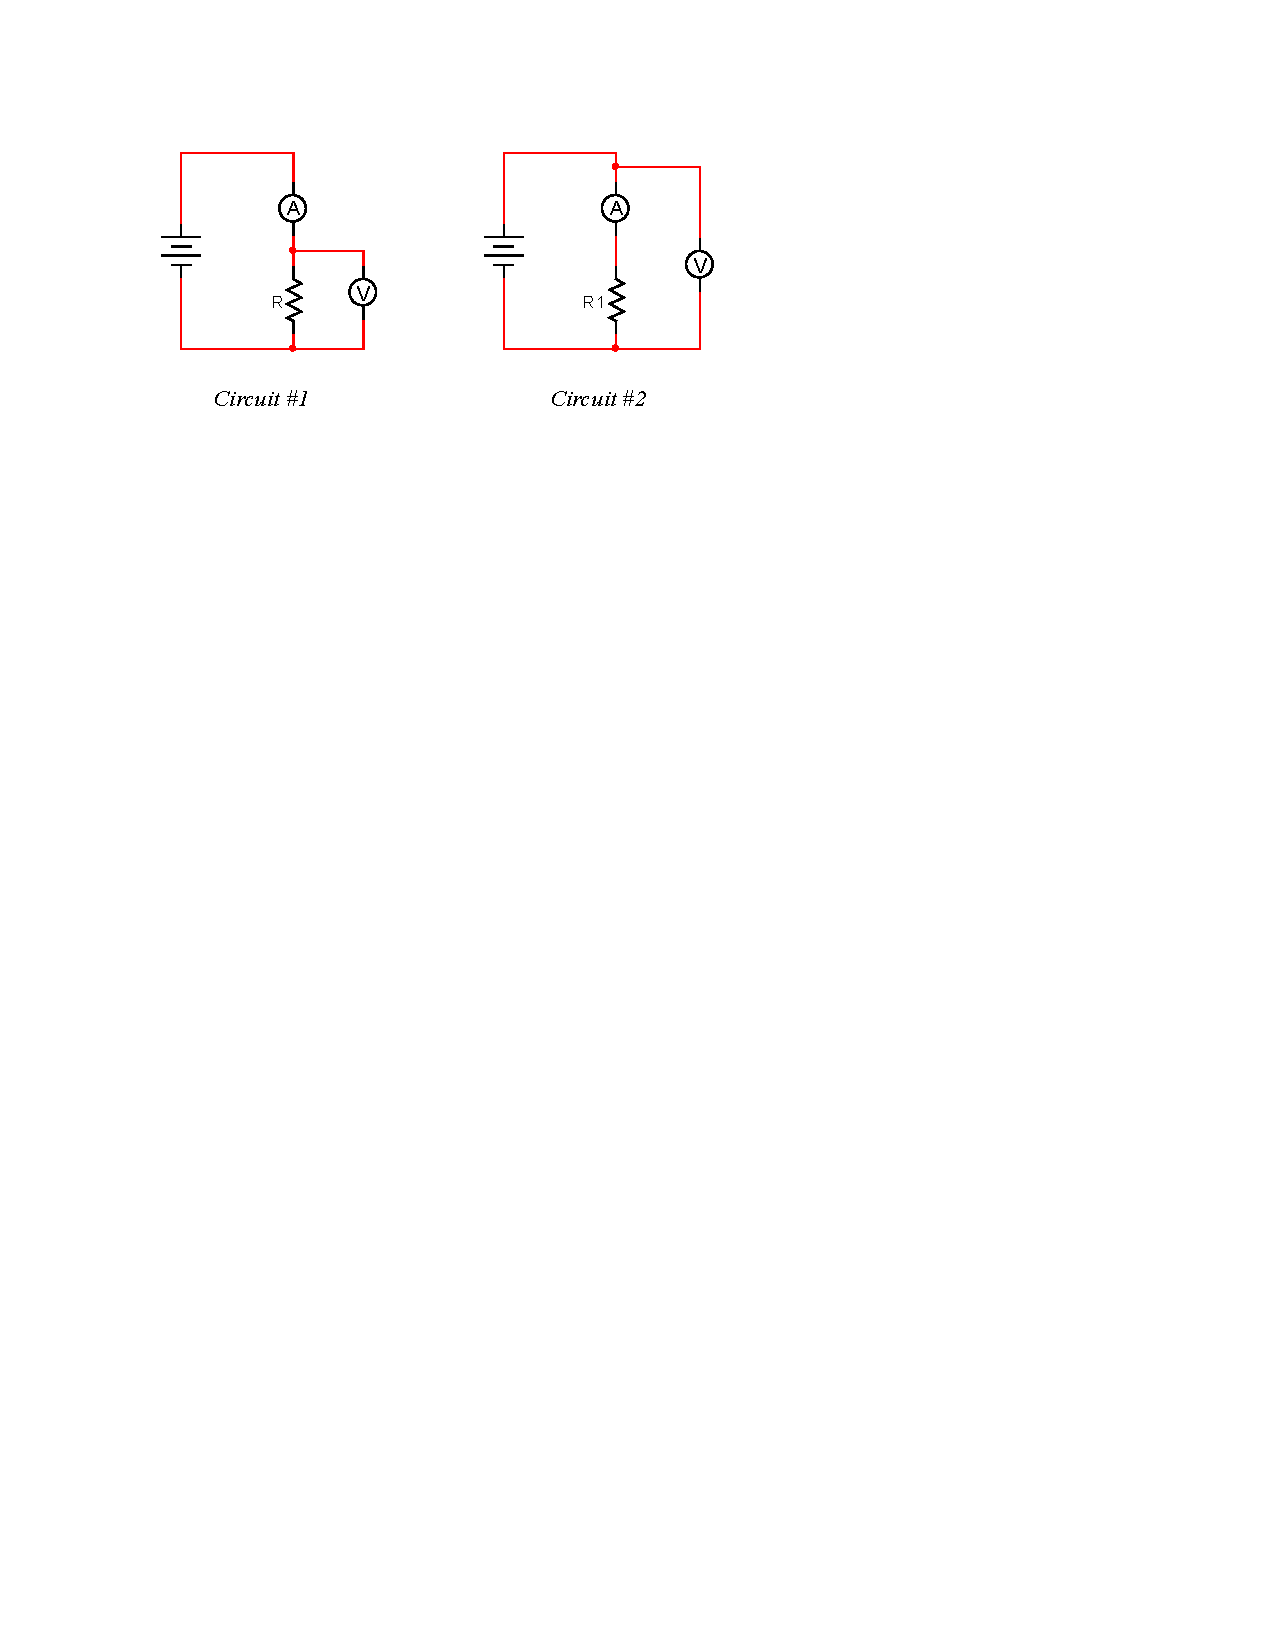
\includegraphics{M_problems/the_basics/I_V_measurements.pdf}
\index{color page}
\end{center}
\end{Exercise}
\begin{Answer}
(a) circuit \#1 (c) circuit \#2 (d) too high (e) circuit \#1
\end{Answer}

%\newcommand{\figuretoright}{3} {%
	%#1 is the picture width
	%#2 is the text to the right


%--------------------------------------------------------------------------------------------------------------
\begin{minipage}[t]{0.7\textwidth}
\begin{Exercise}
As shown in the figure to the right, two resistors in series may be thought of as a \textit{voltage divider}, 
where the output voltage $V_{\rm out}$ is a fixed fraction of the input voltage $V_{\rm in}$.  
Derive a general expression for $V_{\rm out}$ in terms of $R_1$, $R_2$, and $V_{\rm in}$.  Note that the word \textit{derive} means to
demonstrate using some mixture of mathematical statements along with some words and possibly a picture.
\end{Exercise}
\begin{Answer}
$\displaystyle V_{\rm out} = V_{\rm in}\left(\frac{R_2}{R_1+R_2}\right)$.  (Hint: start by finding the current through the resistors.)
\end{Answer}
\end{minipage}
\begin{minipage}[t]{0.3\textwidth - 4pt}

\smallskip
\hfill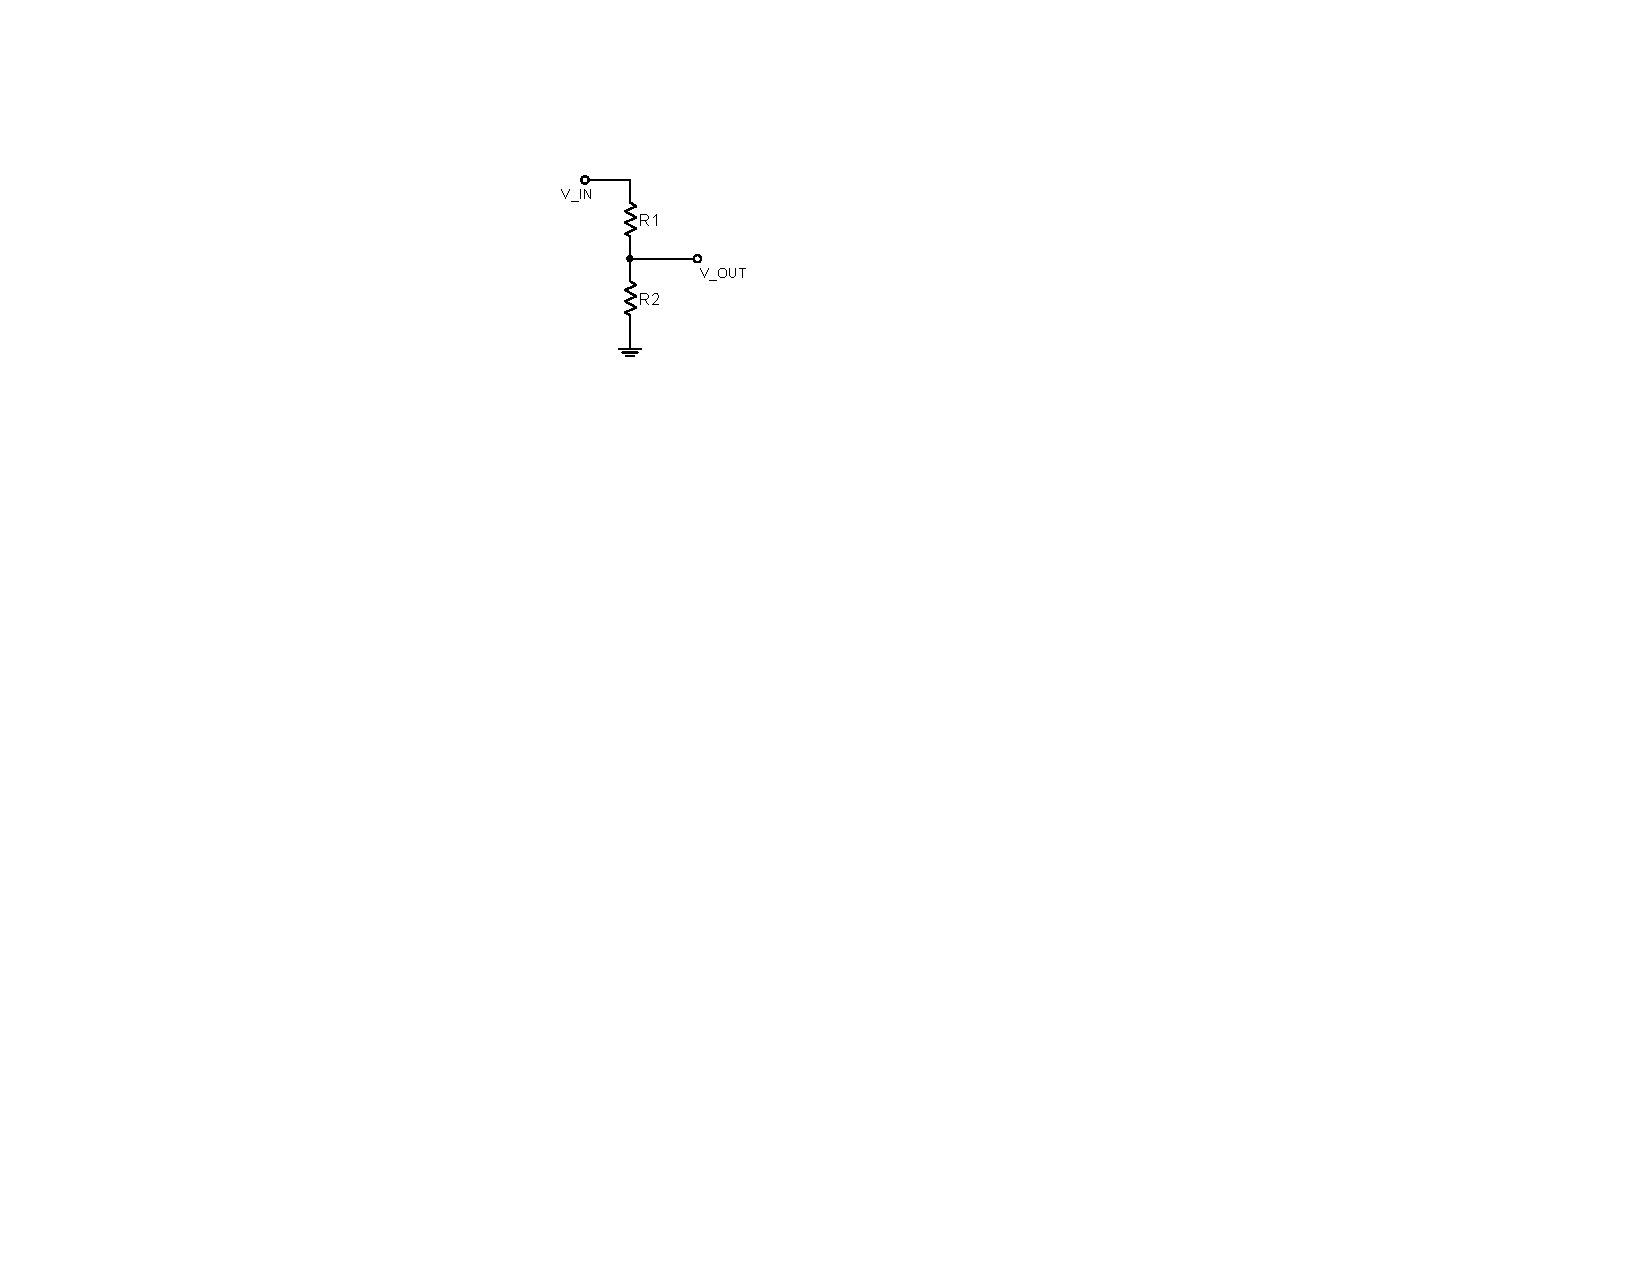
\includegraphics{M_problems/the_basics/voltage_divider.pdf}
\end{minipage}

%--------------------------------------------------------------------------------------------------------------
\begin{Exercise}
\label{prob_impedance_matching}
Consider a power supply like the battery depicted in problem MA2, in which the supply has an internal voltage $\varepsilon$ and an internal resistance $R_{\rm int}$, and where the supply will be connected to a load resistance $R_{\rm load}$.  (Feel free to call the resistances ``$R_1$'' and ``$R_2$'' if you prefer.)
(a)~Write an expression for the power $P_{load}$ dissipated in the load resistor, 
in terms of only $\varepsilon$, $R_{\rm int}$, and $R_{\rm load}$.  
(b)~Suppose that the internal resistance $R_{\rm int}$ of the source is fixed, and you cannot change it.  Derive an expression for the optimal value you should choose for $R_{\rm load}$ in order to \textit{maximize} the power dissipated in the load.
(c)~Now suppose instead that it is the load resistance $R_{\rm load}$ that is fixed and unchangeable.  Derive an expression for the optimal value you should choose for $R_{\rm int}$ in order to \textit{maximize} the power dissipated in the load.
(d)~Based on your answer to part (c), it turns out that some battery types are just better at delivering high load power than others.  Do a little Googling to find how the internal resistance of lithium ion batteries compares to, say, alkaline batteries.  Are there any other battery types that stand out as particularly good or particularly bad?
\end{Exercise}
\begin{Answer}
(b) $R_{\rm load} = R_{\rm int}$ (c) The correct answer is NOT $R_{\rm int} = R_{\rm load}$.
\end{Answer}

%--------------------------------------------------------------------------------------------------------------
\begin{Exercise}
You may have wondered why resistors have the odd values that they often do: for instance, why $2.2\kohm$ and $4.7\kohm$ instead of $2\kohm$ and $5\kohm$? To find out why, check out the Wikipedia entry entitled ``E series of preferred numbers.'' 
\begin{enumerate}[label=(\alph*),nosep]
\item Which set of numbers do the resistors in your kit follow?  (E3? E6? E192?) 
\item In a single sentence of your own words, how are the numbers in that specific sequence calculated?
\end{enumerate}
With the resistors that you have, it is almost always possible to combine just two of them either in series or in parallel to generate virtually any equivalent resistance you want to an accuracy of better than 1\%.  There are various handy online calculators to help you do so, such as the one at \url{https://svajkaj.com/}.  Use this online calculator (or a different one, I guess) to calculate the following:
\begin{enumerate}[resume*]
\item What is the best way to approximate $7.0\kohm$ using just two E6 resistors?
\item What is the best way to approximate $2.7\kohm$ using just two E6 resistors?
\end{enumerate}
\end{Exercise}

%--------------------------------------------------------------------------------------------------------------
\begin{Exercise}
A student has connected the circuit below to their 5~V power supply, expecting a voltmeter reading of $V=2.5$~volts.  Which of the causes listed on the right could lead to each of the symptoms on the left?  More than one answer may apply.

\begin{minipage}[t]{0.35\textwidth}
\textbf{Symptoms}
\begin{enumerate}[nosep,wide]
\item The voltmeter reads 2.58 volts. % i,  within tolerances
\item The voltmeter reads 2.76 volts. % c,  current meter on microvolts
\item The voltmeter reads 4.98 volts. % a,d,e,g  not grounded, or R2 shorted to 5V, or R1 leads touching, or blown fuse. 
\item The voltmeter reads 1.62 volts.  % h, R1 is 10k
\item The voltmeter reads about 0 volts.       % b, R2 shorted 
\end{enumerate}
\end{minipage}%
\begin{minipage}[t]{0.42\textwidth}
\textbf{Causes}
\begin{enumerate}[label=(\alph*),nosep,labelindent=0in]
\item The two leads of $R_1$ are touching each other (``shorted'')
\item The two leads of $R_2$ are touching each other (``shorted'')
\item The current meter is on the $\mu$A scale. 
\item $R_2$ has not been connected to ground.
\item The current meter has a blown fuse.
\item The voltmeter has a blown fuse.
\item One side of $R_2$ has been connected to the 5~V supply.
\item $R_1$ is actually a $10\kohm$ resistor.
\item The circuit is built correctly and the output is within the range expected for the tolerances of the components.
\end{enumerate}
\end{minipage}%
\begin{minipage}[t]{0.22\textwidth}
%Testing testing

\phantom{need text here}

\vspace*{-0.3in}

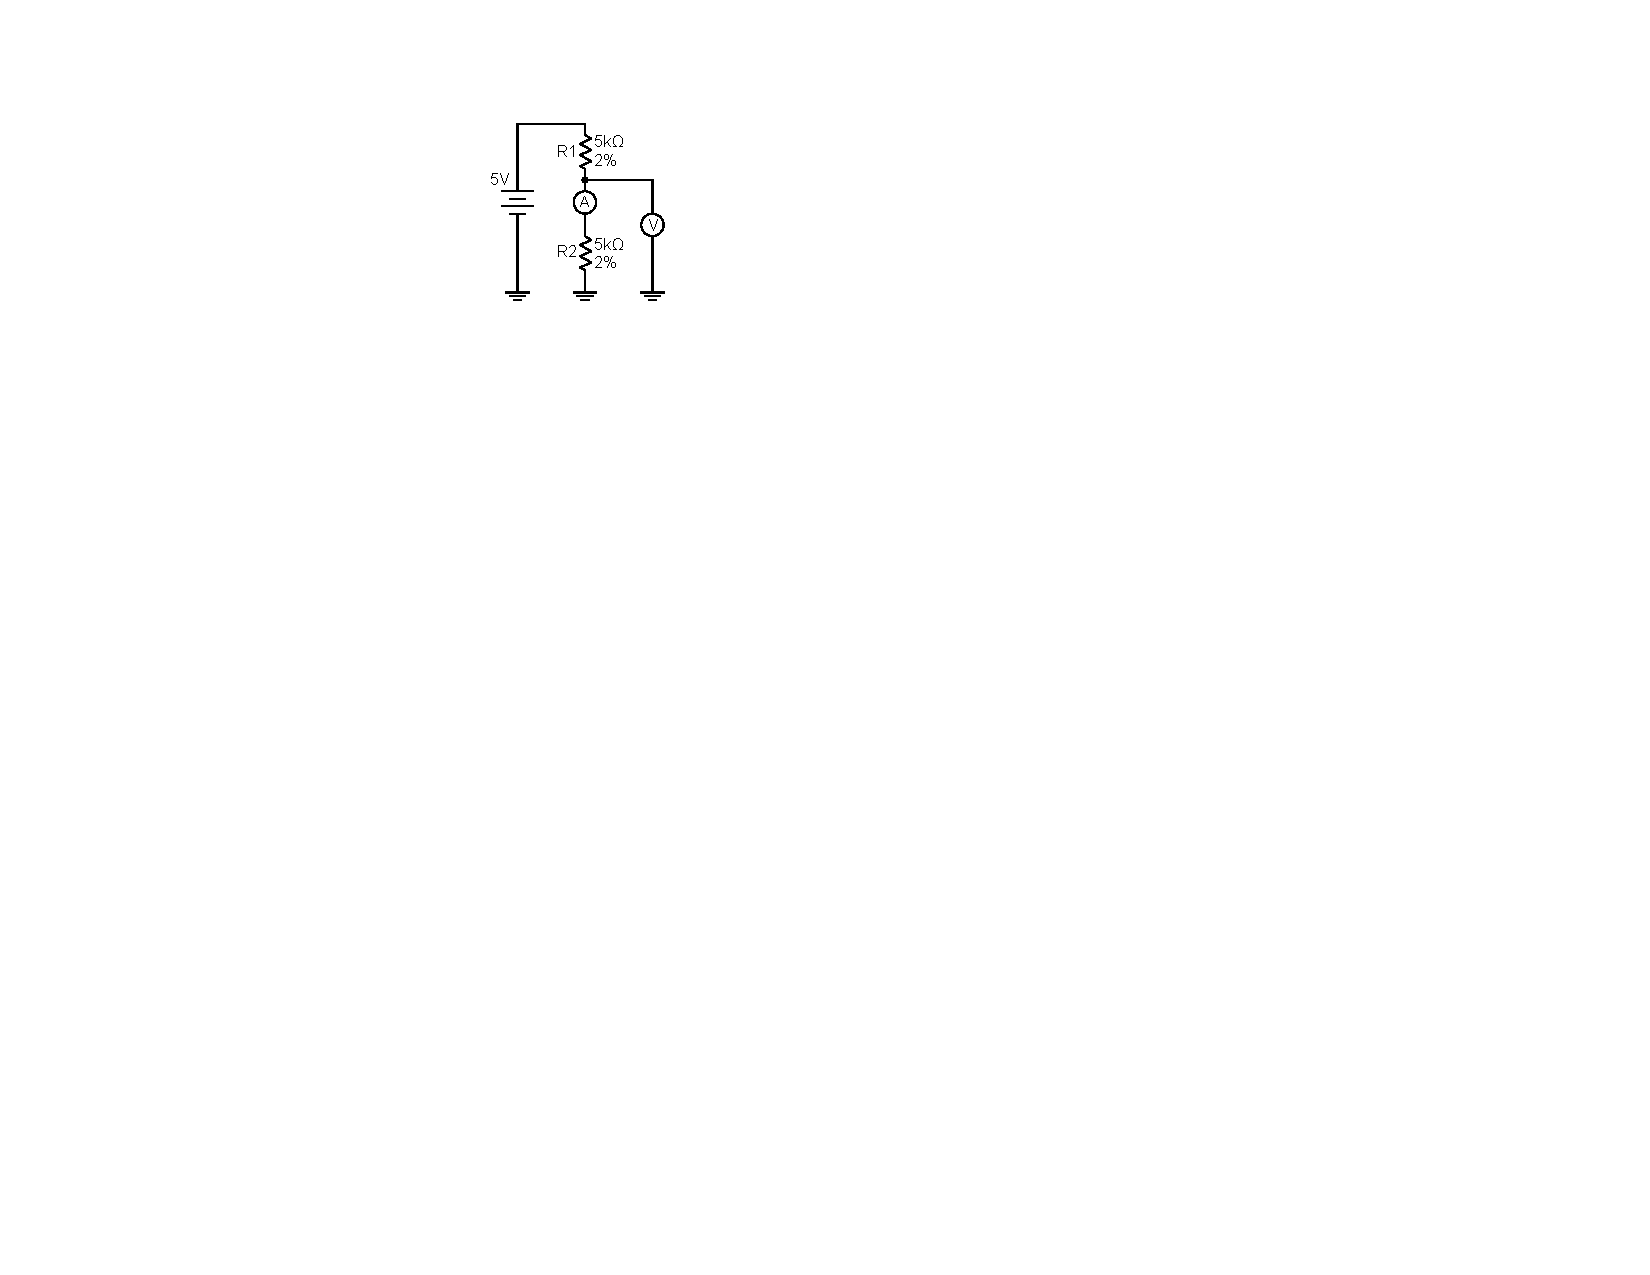
\includegraphics{M_problems/the_basics/troubleshooting_IV_series.pdf}

\end{minipage}%
\end{Exercise}
\begin{Answer}
Of the nine lettered causes (a) thru (i), all but one gets used, and none are used more than once.  Feel free to check your answers for each symptom 1 thru 5 with me; I will tell you what's wrong and let you try again.
\end{Answer}


%--------------------------------------------------------------------------------------------------------------
\begin{Exercise}
A student has constructed the circuit to the right, expecting an adjustable output voltage $V_{\rm out}$ in the range of 2~V to 4~V.  Which of the causes on the right \textit{could} lead to each of the symptoms on the left?  More than one answer may apply.

\begin{minipage}[t]{0.30\textwidth}
\textbf{Symptoms}
\begin{enumerate}[nosep,wide]
\item  $V_{\rm out}$ range is 2~V to 4~V. % g, within tolerances
\item  $V_{\rm out}$ is a constant 6~V.     % a, not grounded
\item  $V_{\rm out}$ is a constant 4~V.     % d, V_out connected to pin 1
\item  $V_{\rm out}$ range is 3~V to 6~V. % b, Two leads of R1 are touching.
\item  $V_{\rm out}$ range is 2~V to 3~V. % e, pins 2 and 3 shorted together.
\item  $V_{\rm out}$ range is 1~V to 2~V. % f, Input voltage is 3 V
\end{enumerate}
\end{minipage}
\begin{minipage}[t]{0.54\textwidth}
\textbf{Causes}
\begin{enumerate}[label=(\alph*),nosep,labelindent=0in]
\item $R_2$ has not been connected to ground. %
\item The two leads of $R_1$ are touching each other.
\item The two leads of $R_2$ are touching each other.
\item $V_{\rm out}$ connected to pin 1, not pin 2.
\item Pins 2 and 3 are connected (``shorted'') together.
\item $V_{\rm in}$ connected to 3 volts.
\item The circuit is correct and the output is within the range expected for the tolerances of the components.
\end{enumerate}
\end{minipage}
\begin{minipage}[t]{0.15\textwidth}

%Testing testing
\phantom{need text here}

\vspace*{-0.3in}

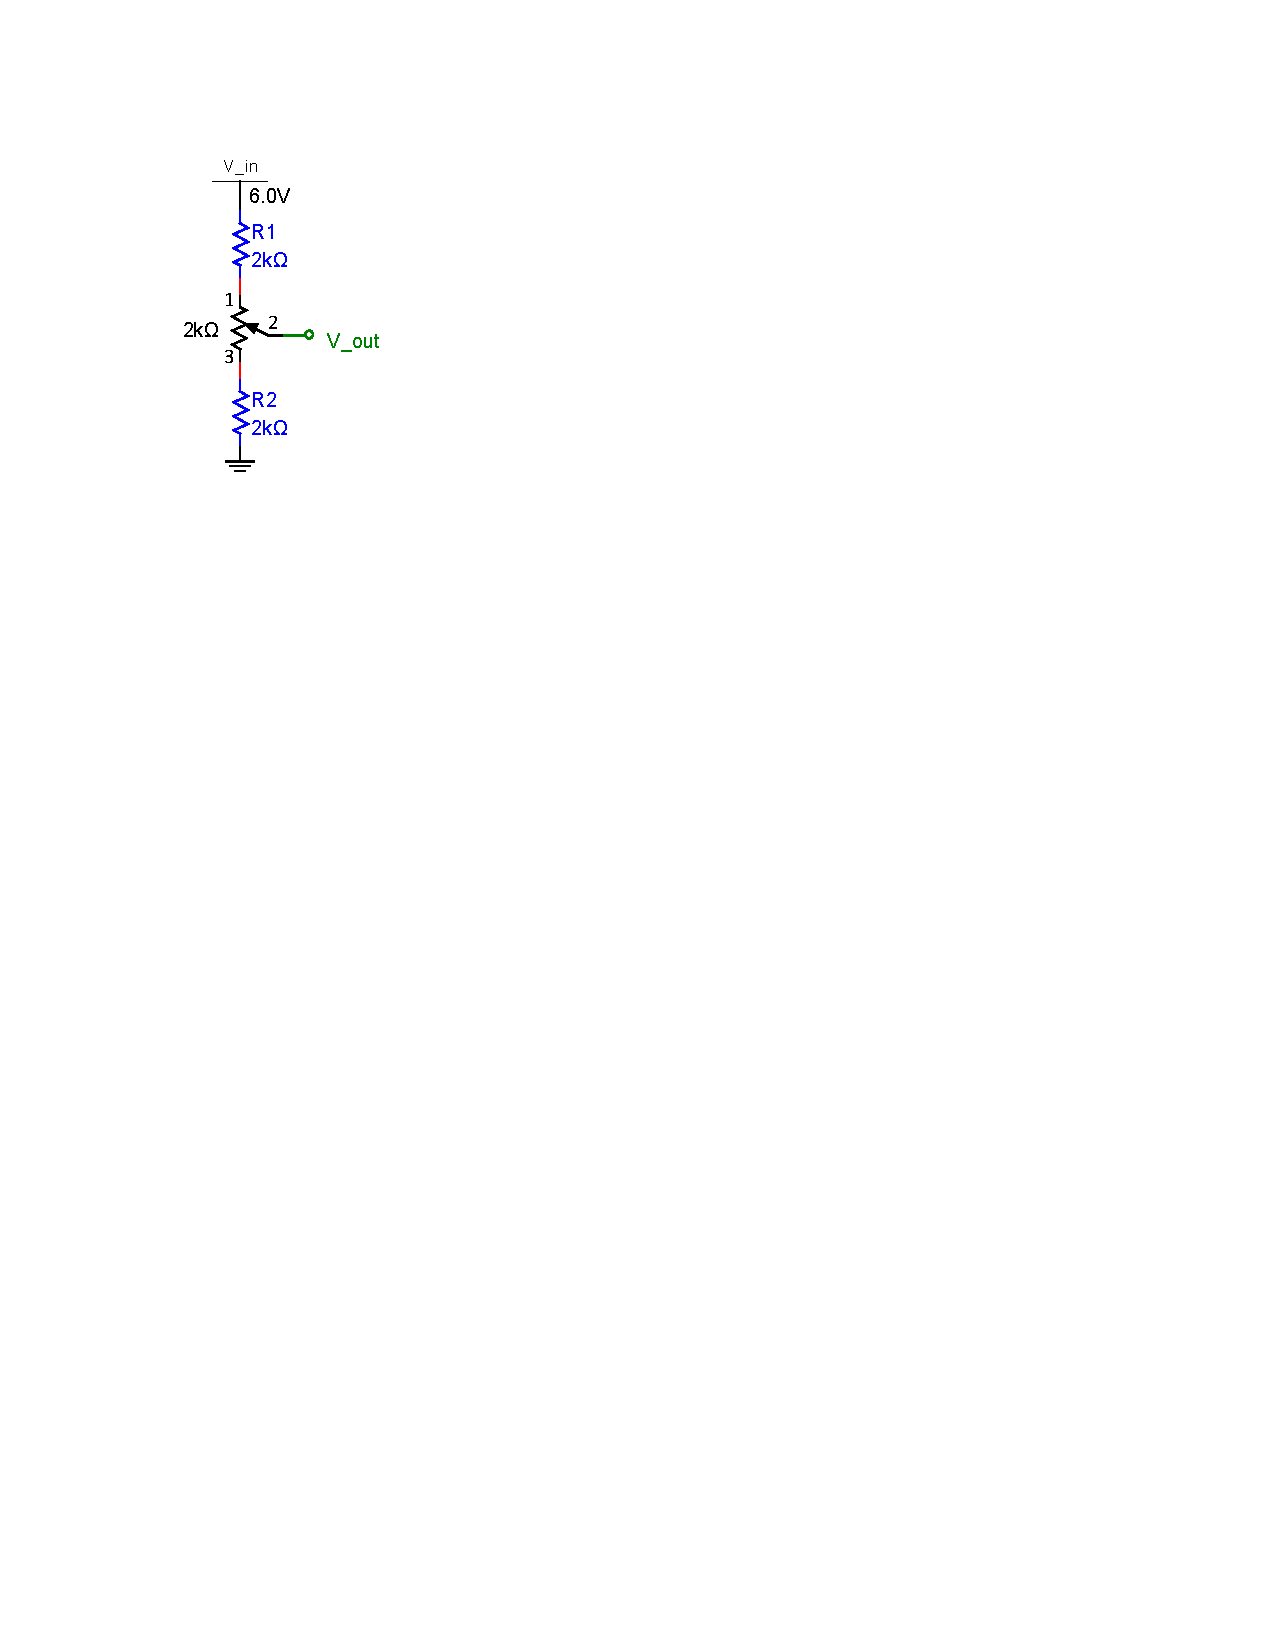
\includegraphics[scale=0.65]{M_problems/the_basics/troubleshooting_voltage_divider_masked.pdf}

\end{minipage}%
\end{Exercise}
\begin{Answer}
Each symptom 1 through 6 has exactly one cause from the list.  Feel free to check your answers for each symptom with me; I will tell you what's wrong and let you try again.
\end{Answer}

%--------------------------------------------------------------------------------------------------------------
\begin{Exercise}
(a)~Design a voltage divider that will guarantee that $V_{\rm out}/V_{\rm in}=0.500$ using a trimpot and two fixed resistors: a $15\kohm$ and $15\kohm$ both 2\% tolerance.  (b)~Design a voltage divider that will guarantee that $V_{\rm out}/V_{\rm in}=1/3$ using a trimpot and two fixed resistors: a $100\kohm$ and $200\kohm$ both 1\% tolerance.  For both parts, use the minimum value of trimpot that will guarantee the correct output.  (Note that ``Design'' means to draw the circuit diagram showing the values of all components.)
\end{Exercise}
\begin{Answer}
(a) $600\ohm$ (b) $4\kohm$
\end{Answer}

%--------------------------------------------------------------------------------------------------------------
\begin{Exercise}
%In this problem, you will examine contact resistance in a trimpot and how to minimize its effects.
A common problem with trimpots and other potentiometers is that the movable wiper (pin 2 in the drawing below) doesn't always make good electrical contact with the resistive material between pins 1 and 3.  The resulting \textit{contact resistance} is particularly pernicious because it can fluctuate wildly over time or when the trimpot is adjusted, leading to effects that are both undesirable and unpredictable.

%pic of contact resistance
\begin{center}
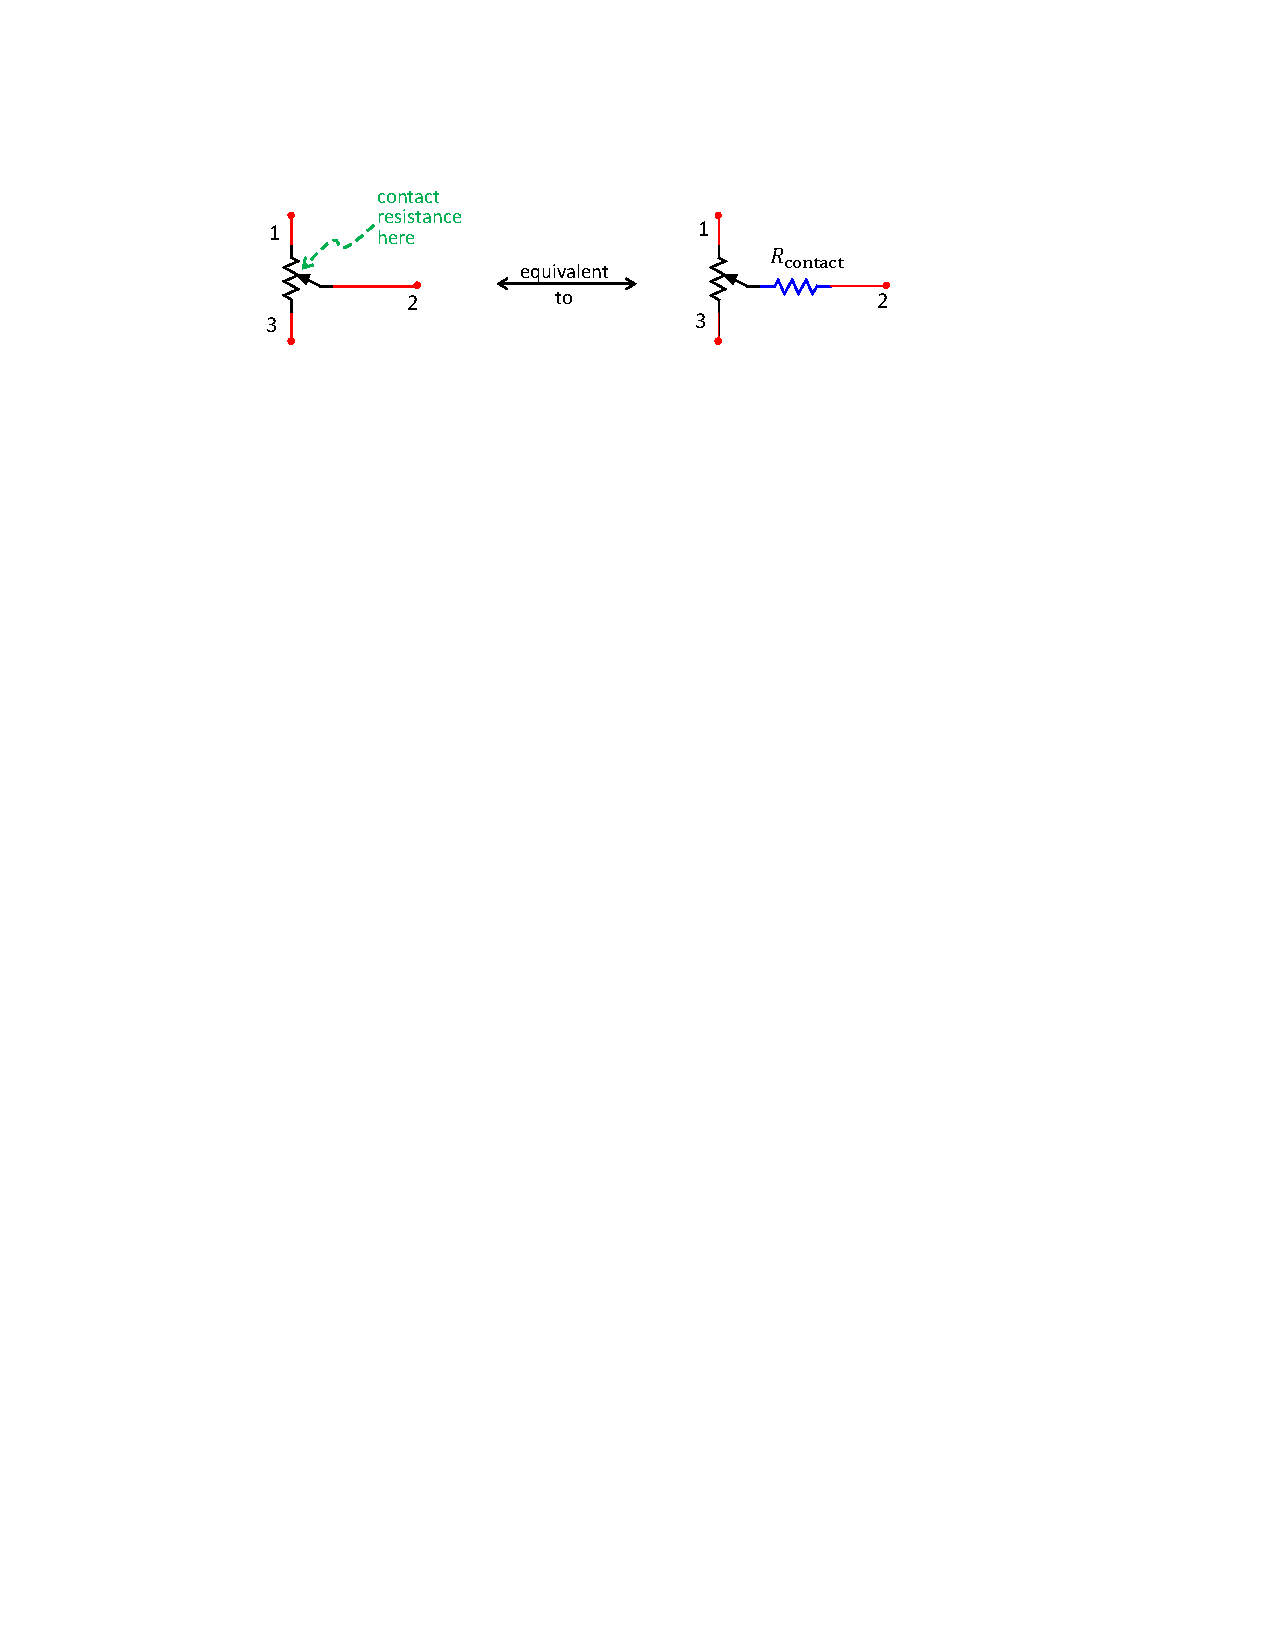
\includegraphics[scale=0.80]{M_problems/the_basics/contact_resistance_defined.pdf}
\end{center}

In the drawing below, the standard way to make a voltage divider is shown in Design~1, on the left.  
\begin{enumerate}[label=(\alph*),nosep]
\item What is the ideal output voltage range for Design~1, assuming that the output is connected to an infinitely large impedance ($R_{\rm load}=\infty$)? (in practice, the output of a voltage divider is almost always connected to something with a high input impedance---think of your voltmeter with $R_{\rm load}=10\Mohm$, for instance.)
\item What is the actual output range for Design~1 if the output is connected to a load with  $R_{\rm load}=1\Mohm$?  
\item How does the actual output range in (b) change with an additional contact resistance $R_{\rm contact}=1\kohm$?  
\end{enumerate}

%pic of three voltage divider circuits
\begin{center}
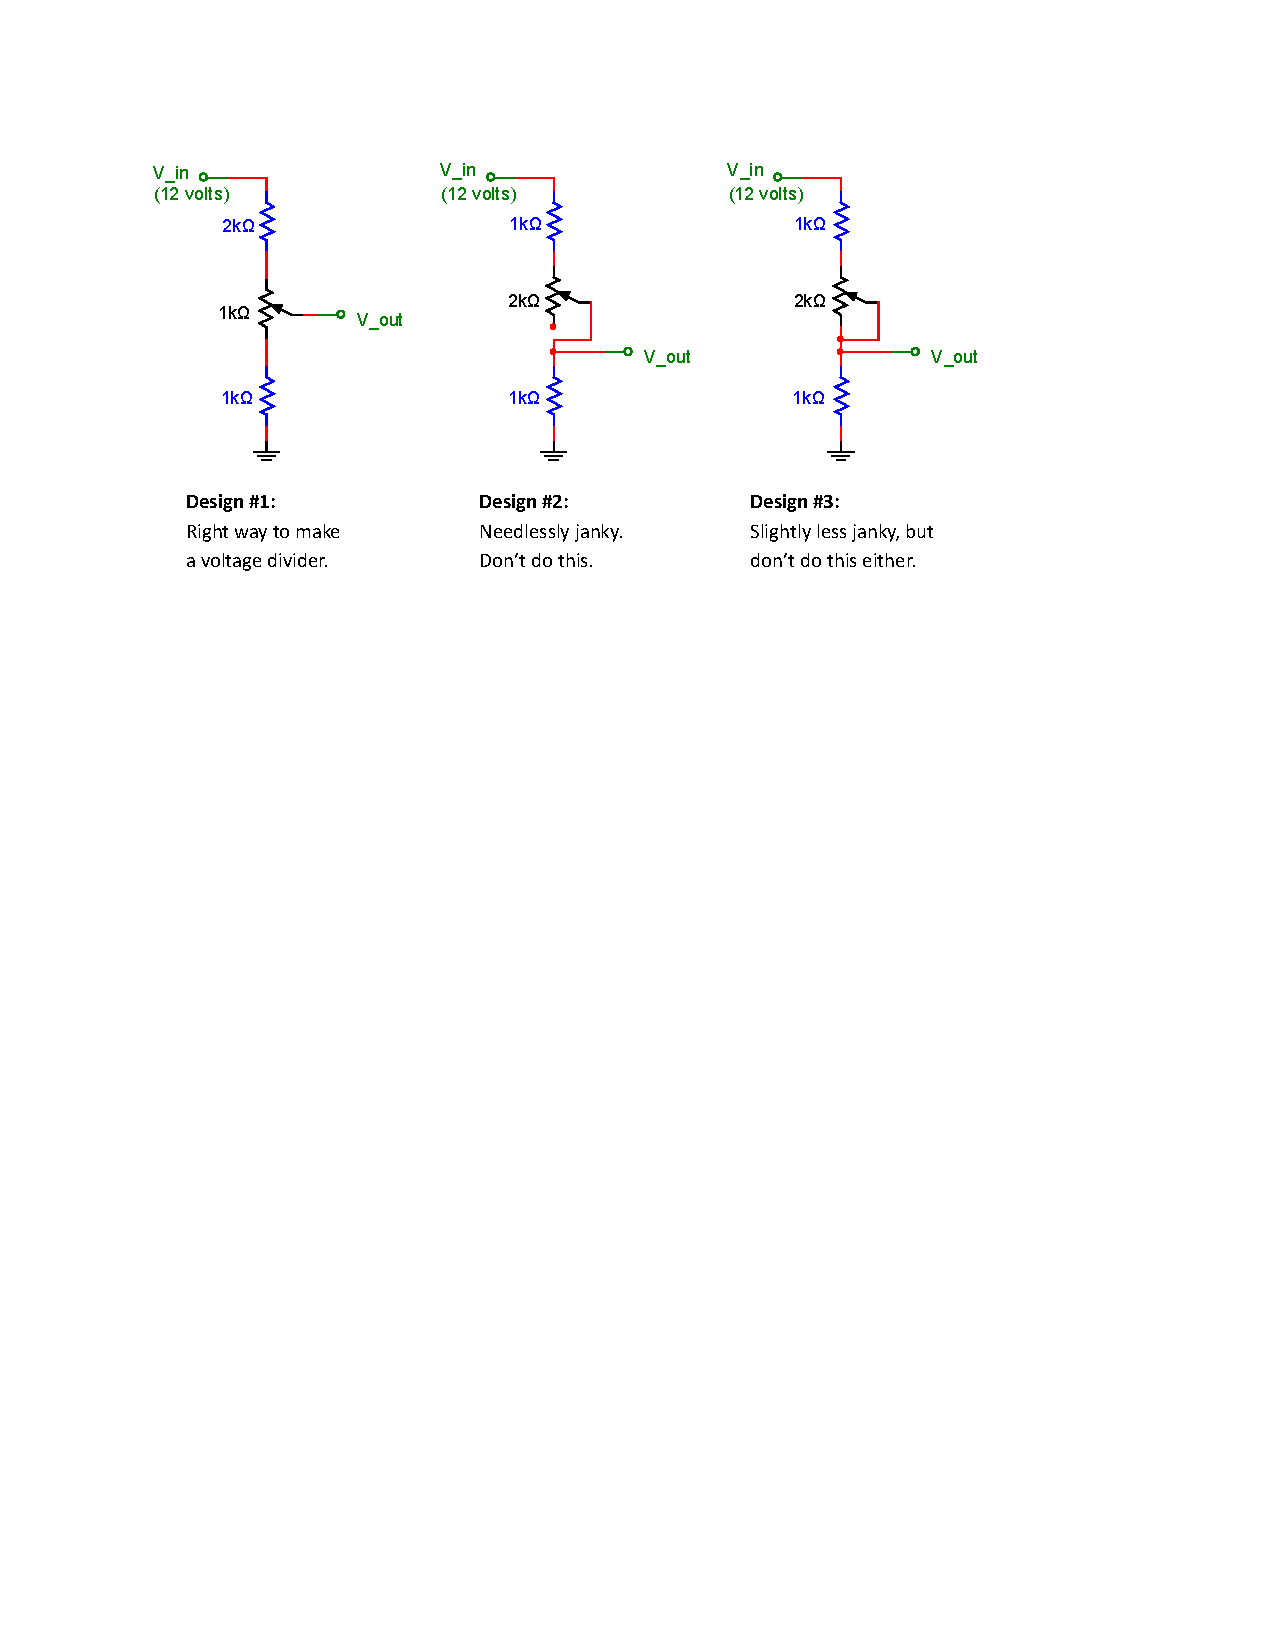
\includegraphics[scale=0.80]{M_problems/the_basics/voltage_divider_contact_resistance.pdf}
\end{center}

Your answers for parts (b) and (c) demonstrate that Design~1 is not affected much by contact resistance.
Designs~2 and~3 above are also ways to build a voltage divider, but
you'll see now that these are much more sensitive to changes in contact resistance.

\begin{enumerate}[resume*]
\item Convince yourself that with with $R_{\rm contact}=0$, Designs~2 and~3 give the same output range as Design~1.  You can assume here and for the remaining parts of this problem that $R_{\rm load}=\infty$.
\item What is the output range for Design~2 with $R_{\rm contact}=1\kohm$? What about with $R_{\rm contact}=\infty$?
\item What is the output range for Design~3 with $R_{\rm contact}=1\kohm$? What about with $R_{\rm contact}=\infty$?
\item Why is Design~3 better than Design~2?
\end{enumerate}
In general, you want as little current as possible to flow through the wiper of a potentiometer, to minimize the effect of contact resistance.  You very rarely need to use a potentiometer as a two-terminal variable resistor, but if you do you should always connect the wiper lead to one of the outer leads as in Design 3.
\end{Exercise}
\begin{Answer}
(a)~3.0 to 6.0~volts.  \\
(b)~$2.997\,751\,686$ to $5.994\,005\,994$~volts. ($R_{\rm load}$ changes the output voltages by about 0.1\%.)\\
(c)~$2.997\,753\,931$ to $5.994\,011\,976$~volts. ($R_{\rm contact}$ changes the output voltages by about 0.0001\%.)\\
(e)~2.4 to 4.0~volts for $R_{\rm contact} =1\kohm$, or constant 0~V for $R_{\rm contact} =\infty$.\\
(f)~3.0 to 4.5~volts for $R_{\rm contact} =1\kohm$, or constant 3~V for $R_{\rm contact} =\infty$.\\
(g)~With contact resistance, output of Design 3 is always closer to intended range than Design 2.  In fact, the output of Design 3 will never be \textit{outside} of the intended range, though the full intended range may not be accessible.
\end{Answer}

%--------------------------------------------------------------------------------------------------------------
\begin{Exercise}
A sinusoidal voltage with an amplitude of 10~V and a frequency of 0.25~Hz is placed across a load resistance of $220\ohm$.  (a)~What is the maximum \textit{instantaneous} power dissipated in the resistor?  (b) What is the \textit{average} power dissipated in the resistor?
\end{Exercise}
\begin{Answer}
(a) 0.45 W (b) 0.23 W
\end{Answer}

%--------------------------------------------------------------------------------------------------------------
\begin{Exercise}
The periodic waveform shown below is 20~V for $10~\mu$s and $-5$~V for $15~\mu$s.
\begin{center}
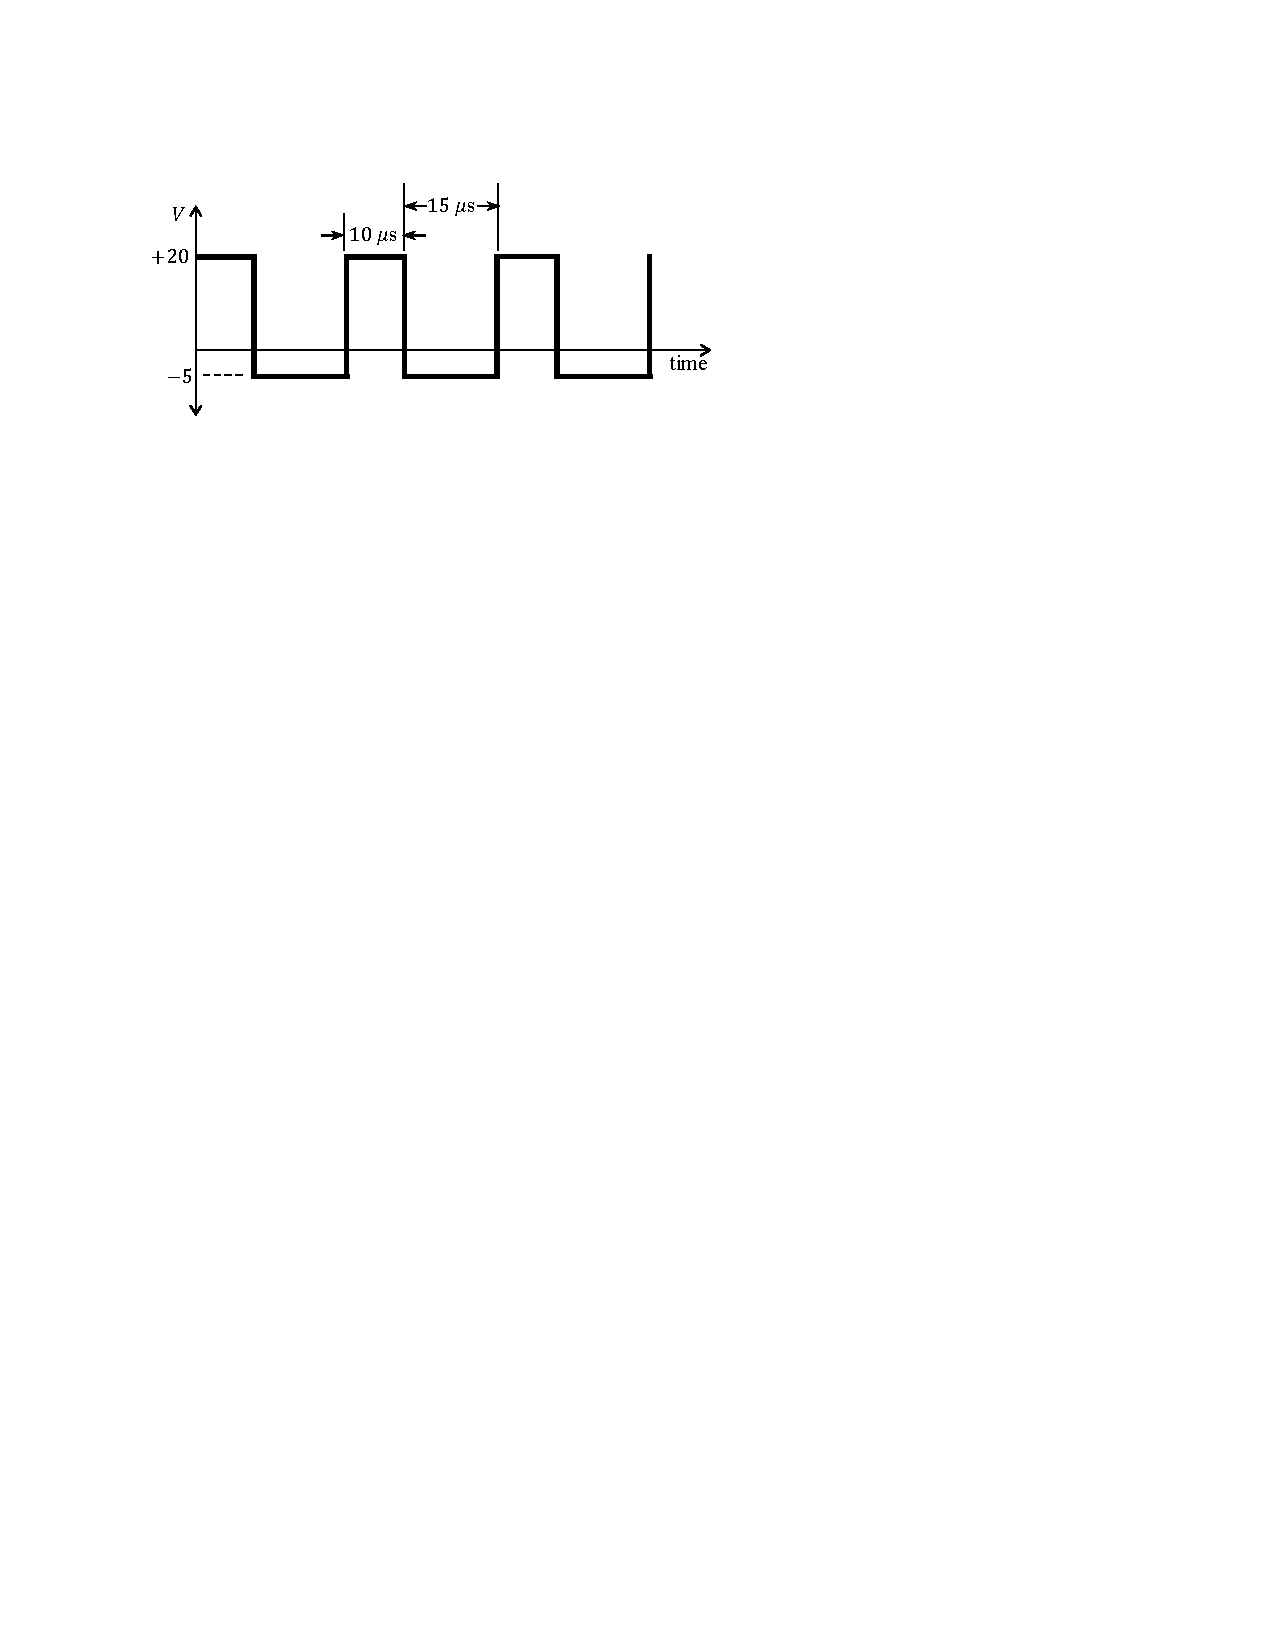
\includegraphics{M_problems/the_basics/irregular_periodic_wave.pdf}
\end{center}

\begin{enumerate}[label=(\alph*),nosep]
\item What range of voltages is displayed on an oscilloscope if the signal is measured using DC coupling?
\item What range of voltages is displayed on an oscilloscope if the signal is measured using AC coupling?
\item What is the RMS value of this signal as measured using DC coupling?
\item What is the RMS value of this signal as measured using AC coupling?
\end{enumerate}
\end{Exercise}
\begin{Answer}
(b)$-10$ to 15 V (c)~13.23~V (d)~12.25~V 
\end{Answer}

%--------------------------------------------------------------------------------------------------------------
\begin{Exercise}
(a)~Find the RMS voltage of a periodic sawtooth wave which rises linearly from 0 to $V_{\rm max}$ and falls instantaneously to zero, such that $V=V_{\rm max}t/\tau$, where $\tau$ is the period.  Yes, you will need to compute an integral to answer this question. 
(b)~Use your result from part (a) to find the RMS voltage of a triangle wave (as from your function generator) that oscillates between $-V_{\rm peak}$ and $+V_{\rm peak}$.
\end{Exercise}
\begin{Answer}
(a) $0.58V_{\rm max}$
\end{Answer}

%Ideas for additional problems:
%uncertainty, like 132 problem?
%pictures of breadboards with resistors, where students draw circuit diagram or say if resistors are in parallel or series

%\vfill
%\pagebreak[3]

\vspace{0.7in}

\textbf{Answers to Selected {\thesubsection} Problems:}
\label{the_basics_prob_answers}
%\shipoutExercise
\shipoutAnswer

\cleardoublepage
